\documentclass[12pt,twoside]{article}
%%%%%%%%%%%%%%%%%%%%%%%%%%%%%%%%%%%%%%%%%%%%%%%%%%%%%%%%%%%%%
% Meta informations:
\newcommand{\trauthor}{Weipeng He}
\newcommand{\trtype}{Seminar Paper} %{Seminararbeit} %{Proseminararbeit}
\newcommand{\trcourse}{Bio-inspired Artificial Intelligence}
\newcommand{\trtitle}{Self-replicating Robots : A review}
\newcommand{\trmatrikelnummer}{6411529}
\newcommand{\tremail}{2he@informatik.uni-hamburg.de}
\newcommand{\trarbeitsbereich}{Knowledge Technology, WTM}
\newcommand{\trdate}{\today}

%%%%%%%%%%%%%%%%%%%%%%%%%%%%%%%%%%%%%%%%%%%%%%%%%%%%%%%%%%%%%
% Languages:

% Falls die Ausarbeitung in Deutsch erfolgt:
% \usepackage[german]{babel}
% \usepackage[T1]{fontenc}
% \usepackage[latin1]{inputenc}
% \usepackage[latin9]{inputenc}	 				
% \selectlanguage{german}

% If the thesis is written in English:
\usepackage[english]{babel} 						
\selectlanguage{english}

%%%%%%%%%%%%%%%%%%%%%%%%%%%%%%%%%%%%%%%%%%%%%%%%%%%%%%%%%%%%%
% Bind packages:
\usepackage{acronym}                    % Acronyms
\usepackage{algorithmic}								% Algorithms and Pseudocode
\usepackage{algorithm}									% Algorithms and Pseudocode
\usepackage{amsfonts}                   % AMS Math Packet (Fonts)
\usepackage{amsmath}                    % AMS Math Packet
\usepackage{amssymb}                    % Additional mathematical symbols
\usepackage{amsthm}
\usepackage{booktabs}                   % Nicer tables
%\usepackage[font=small,labelfont=bf]{caption} % Numbered captions for figures
\usepackage{color}                      % Enables defining of colors via \definecolor
\definecolor{uhhRed}{RGB}{254,0,0}		  % Official Uni Hamburg Red
\definecolor{uhhGrey}{RGB}{122,122,120} % Official Uni Hamburg Grey
\usepackage{fancybox}                   % Gleichungen einrahmen
\usepackage{fancyhdr}										% Packet for nicer headers
%\usepackage{fancyheadings}             % Nicer numbering of headlines

%\usepackage[outer=3.35cm]{geometry} 	  % Type area (size, margins...) !!!Release version
%\usepackage[outer=2.5cm]{geometry} 		% Type area (size, margins...) !!!Print version
%\usepackage{geometry} 									% Type area (size, margins...) !!!Proofread version
\usepackage[outer=3.15cm]{geometry} 	  % Type area (size, margins...) !!!Draft version
\geometry{a4paper,body={5.8in,9in}}

\usepackage{graphicx}                   % Inclusion of graphics
%\usepackage{latexsym}                  % Special symbols
\usepackage{longtable}									% Allow tables over several parges
\usepackage{listings}                   % Nicer source code listings
\usepackage{multicol}										% Content of a table over several columns
\usepackage{multirow}										% Content of a table over several rows
\usepackage{rotating}										% Alows to rotate text and objects
\usepackage[hang]{subfigure}            % Allows to use multiple (partial) figures in a fig
%\usepackage[font=footnotesize,labelfont=rm]{subfig}	% Pictures in a floating environment
\usepackage{tabularx}										% Tables with fixed width but variable rows
\usepackage{url,xspace,boxedminipage}   % Accurate display of URLs

%%%%%%%%%%%%%%%%%%%%%%%%%%%%%%%%%%%%%%%%%%%%%%%%%%%%%%%%%%%%%
% Configurationen:

\hyphenation{whe-ther} 									% Manually use: "\-" in a word: Staats\-ver\-trag

%\lstloadlanguages{C}                   % Set the default language for listings
\DeclareGraphicsExtensions{.pdf,.svg,.jpg,.png,.eps} % first try pdf, then eps, png and jpg
\graphicspath{{./data/}} 								% Path to a folder where all pictures are located
\pagestyle{fancy} 											% Use nicer header and footer

% Redefine the environments for floating objects:
\setcounter{topnumber}{3}
\setcounter{bottomnumber}{2}
\setcounter{totalnumber}{4}
\renewcommand{\topfraction}{0.9} 			  %Standard: 0.7
\renewcommand{\bottomfraction}{0.5}		  %Standard: 0.3
\renewcommand{\textfraction}{0.1}		  	%Standard: 0.2
\renewcommand{\floatpagefraction}{0.8} 	%Standard: 0.5

% Tables with a nicer padding:
\renewcommand{\arraystretch}{1.2}

%%%%%%%%%%%%%%%%%%%%%%%%%%%%
% Additional 'theorem' and 'definition' blocks:
\theoremstyle{plain}
\newtheorem{theorem}{Theorem}[section]
%\newtheorem{theorem}{Satz}[section]		% Wenn in Deutsch geschrieben wird.
\newtheorem{axiom}{Axiom}[section] 	
%\newtheorem{axiom}{Fakt}[chapter]			% Wenn in Deutsch geschrieben wird.
%Usage:%\begin{axiom}[optional description]%Main part%\end{fakt}

\theoremstyle{definition}
\newtheorem{definition}{Definition}[section]

%Additional types of axioms:
\newtheorem{lemma}[axiom]{Lemma}
\newtheorem{observation}[axiom]{Observation}

%Additional types of definitions:
\theoremstyle{remark}
%\newtheorem{remark}[definition]{Bemerkung} % Wenn in Deutsch geschrieben wird.
\newtheorem{remark}[definition]{Remark} 

%%%%%%%%%%%%%%%%%%%%%%%%%%%%
% Provides TODOs within the margin:
\newcommand{\TODO}[1]{\marginpar{\emph{\small{{\bf TODO: } #1}}}}

%%%%%%%%%%%%%%%%%%%%%%%%%%%%
% Provides latin abbriviations:
\newcommand{\etal}{\textit{et al.}}
\newcommand{\etc}{\textit{etc.}}
\newcommand{\eg}{\textit{e.g.}}

%%%%%%%%%%%%%%%%%%%%%%%%%%%%
% Abbreviations and mathematical symbols
\newcommand{\modd}{\text{ mod }}
\newcommand{\RS}{\mathbb{R}}
\newcommand{\NS}{\mathbb{N}}
\newcommand{\ZS}{\mathbb{Z}}
\newcommand{\dnormal}{\mathit{N}}
\newcommand{\duniform}{\mathit{U}}

\newcommand{\erdos}{Erd\H{o}s}
\newcommand{\renyi}{-R\'{e}nyi}
%%%%%%%%%%%%%%%%%%%%%%%%%%%%%%%%%%%%%%%%%%%%%%%%%%%%%%%%%%%%%
% Document:
\begin{document}
\renewcommand{\headheight}{14.5pt}

\fancyhead{}
\fancyhead[LE]{ \slshape \trauthor}
\fancyhead[LO]{}
\fancyhead[RE]{}
\fancyhead[RO]{ \slshape \trtitle}

%%%%%%%%%%%%%%%%%%%%%%%%%%%%
% Cover Header:
\begin{titlepage}
	\begin{flushleft}
		Universit\"at Hamburg\\
		Department Informatik\\
		\trarbeitsbereich\\
	\end{flushleft}
	\vspace{3.5cm}
	\begin{center}
		\huge \trtitle\\
	\end{center}
	\vspace{3.5cm}
	\begin{center}
		\normalsize\trtype\\
		[0.2cm]
		\Large\trcourse\\
		[1.5cm]
		\Large \trauthor\\
		[0.2cm]
		\normalsize Matr.Nr. \trmatrikelnummer\\
		[0.2cm]
		\normalsize\tremail\\
		[1.5cm]
		\Large \trdate
	\end{center}
	\vfill
\end{titlepage}

	%backsite of cover sheet is empty!
\thispagestyle{empty}
\hspace{1cm}
\newpage

%%%%%%%%%%%%%%%%%%%%%%%%%%%%
% Abstract:

% Abstract gives a brief summary of the main points of a paper:
\section*{Abstract}
In the past few years, the field of self-replicating robotics has advanced from proof-of-concept systems to physical implementations. This technology of imitating living organisms has many important applications as well as Platonic appeal for scientist.

In this review paper, we discuss the recent studies on self-replicating robotics. We categorize those techniques to three different types: directed replication via fabrication, directed replication via module assembly, self-assembly of randomly agitated modules. These different approaches are evaluated.

% Lists:
\tableofcontents
\pagenumbering{arabic}
\clearpage

%%%%%%%%%%%%%%%%%%%%%%%%%%%%
% Content:

% the actual content, usually separated over a number of sections
% each section is assigned a label, in order to be able to put a
% crossreference to it

\section{Introduction}
\label{sec:intro}

\subsection{Self-replication and self-reproduction}
Self-replication is the process of a machine autonomously creating an identical functional copy of itself. The concept of self-replication is inspired by the reproduction process of living organism. Thus, the study of self-replicating machines is intriguing for its romantic and Platonic idea of making artificial machines which can imitate the real live.

The reproduction process in nature, however, does not make the identical copy of the parent(s). Namely, the reproduction contains error, which might be good or not. So is the concept of self-reproduction machines, which is also a topic for computer scientists. The self-reproduction is the process of a machine autonomously creating an approximate copy of itself.

Worth to mention is that, as stated in The Second Law of Thermodynamics and Shannon's theorem about information, it is impossible to copy information without any loss. Therefore, we consider the replica of replication can be within specified tolerances that
will work as well as the original\cite{jones_reprap_2011}.

\subsection{Self-replicating robots}
Research in self-replication was introduced by John von Neumann\cite{von_neumann_theory_1962} more than 60 years ago. Yet it was not until last decade that researchers implemented physical self-replicating robots\cite{suthakorn_autonomous_2003}. 

The applications for self-replication also break through from theoretical work to practical projects. Originally proposed in a NASA project of advanced automation for space missions \cite{freitas_report_1981}, the applications of self-replicating robots for space exploration and development have been promoted by recent achievements of physically realized self-replicating robots\cite{chirikjian_self-replicating_2002}. The exponential growth of self-replicating robots can minimize the launch payload and free human from working on-site.

Although many excellent works in theoretical self-replicating machines, especially in cellular automata, are studied by scientist, in this paper we only focus on those designs that have already been physically implemented or at least are apparently easy to realize.

\subsection{Categorization}
Lee \etal\cite{lee_robotic_2008} classified the recent work on self-replicating robots into four categories. We adopted three of them, which will be discussed in this review paper :

  \emph{Directed replication via fabrication}: Using rapid prototyping technology, a 3-D printer make a replica of itself out of raw material.
  
  \emph{Directed replication via module assembly}: A modular robot executes a directed sequence of movement to assemble prepared spare modules to a replica robot.
  
  \emph{Self-assembly of randomly agitated modules}: Modules are kept moving randomly in a environment with external work source, and then assemble to functional parts through a stochastic process.

We exclude the category, self-reconfigurable modular robots, for the reason that it is not close related to the topic of self-replication. Although some technology of self-reconfigurable modular robots are basics for self-replicable modular robots, the self-reconfigurable modular robots are not necessarily to be able to replicate.

\subsection{Attributes for self-replicating robots}
For evaluating the quality of a self-replicating robots, we discuss the following attributes, which are closely related to the implementation and application for self-replicating robots:

\emph{Accessibility of raw materials}: For the replication process, there must be physical input, which is the raw materials. The raw materials can be spare robot modules, plastic, metal or substance from nature. We expect the robots can take materials of higher accessibility as the input, so that the robots have higher adaptation in the environment. However, using nature substance as raw material is still an ideal goal for the researchers. So far, we consider those self-replicating robots that use plastic and metal as raw materials are better than those use complex spare robot modules.
  
\emph{Artificial level of environment}: Robots work in different environments. Some are artifical set up, while other are not. According to it artificial level, the working environment can be categorized in three level\cite{lee_robotic_2007} : structured environment, semi-structured environment and unstructured environment. In structured environment, objects are placed in exact precise location with predefined order. In semi-structured or partially structured environment, objects are placed in exact location with small error and random order. An unstructured environment is without any structure resulting from initial human intervention.
  
\emph{Autonomy of design}: While the replication process of robots can be totally designed by developers, it is also possible to use evolution algorithm for the design with less predefined knowledge. The evolution ability will be quite essential in future designs as both the structures of the robots and the environment will be more complex, which make it more difficult for researchers to find out a proper procedure for replication.

% \emph{Degree of complexity}: Both Lee \etal\cite{lee_robotic_2008} and Adams \etal\cite{adams_universal_2009} proposed methods to measure the degree of complexity of the replication process. \TODO{}
% 
% \subsection{Difficulties in self-replicating robots}
% \TODO{} 

\section{Directed replication via fabrication}
\label{sec:fabri}

As mentioned before, we can directly use rapid prototypers to manufacture the copy of the machines themselves. Examples are RepRap machine\cite{jones_reprap_2011}, cyclic fabrication system(CFS)\cite{moses_towards_2009} and Fab@Home machine\cite{malone_fabhome:_2007}.

\subsection{Rapid prototypers}
Rapid prototypers or 3D printers are machines that can rapidly fabricate objects on demand from computer-generated design specifications(such as CAD models)\cite{lipson_homemade_2005}. These prototypers usually take thermoplastic polymers as the raw materials. Either addition techniques (aggregation of melted plastics) or subtraction techniques (sculpture from a piece of raw plastics) is used to get the specified shape.

In the past 30 years, rapid prototyping have been favored by the manufacturing industry, as such technologies can enormously shorten the design period of new products. Recently, scientists made it possible to use prototypers at laboratories or at home.

\subsection{RepRap : an example}
RepRap is an open-source project for self-replicating rapid prototyping machines\cite{jones_reprap_2011} (see figure \ref{fig:reprap}). The machine adopted fused-filament
fabrication as the core technique to make product from thermoplastic polymers.
RepRap is one of the state-of-the-art self-replicating fabricators, as it is capable to create most of its own part, while the rest part are components which are relatively easy to make or to purchase from the market.

\begin{figure}[hbtp]
	 \centerline{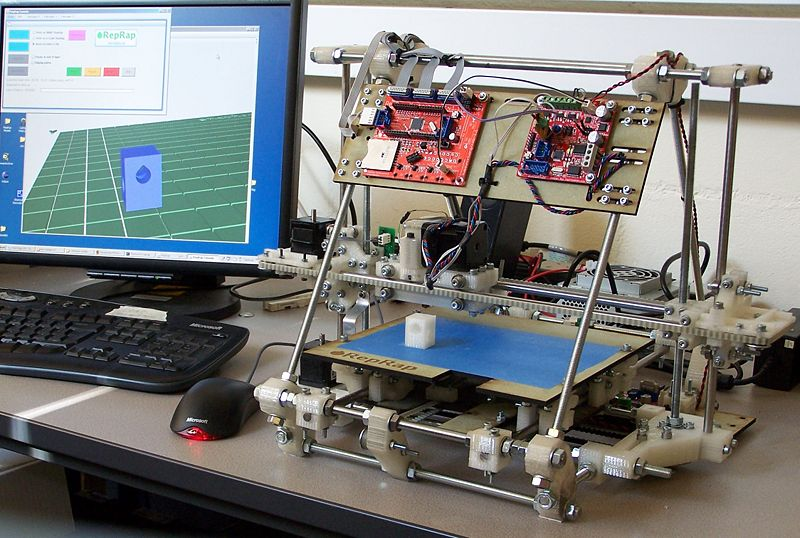
\includegraphics[width=0.7\textwidth]{mendel}}
	 {\caption{RepRap Version II ``Mendel'' (from \cite{jones_reprap_2011})}
	 \label{fig:reprap}}
\end{figure}

Different from other rapid prototyper, RepRap adapted several features to make the machine itself simple enough to self-manufacture. RepRap machine are designed to be small and light weight. Most of building materials are polylactic acid(PLA), which is hard, resistant to contraction problems on cooling and has medium melding point. RepRap also avoids complicated components, such as laser and inkjet print head, in its design.

As reported by the authors, the second version of RepRap machine can produce up to 57\% of its own part. The number of RepRap machines are estimated to be increased from 4 to 4500 via self-replication in 2 and half years(from 2008 to 2011). The success in growth of number of derived copies also indicates that the child machine are made within the tolerance of error.

While the machine is capable to create its consisting components, it cannot autonomously assemble the produced parts. As a matter of fact, the machine are assembled with manual assistance. Of course, the autonomous assembly, which is another field of study, can be applied.

\section{Directed replication via module assembly}
\label{sec:module}
Directed replication via module assembly is an approach to self-replication from another aspect. Other than focusing on fabrication, studies on these types of robots focus on autonomous assembly of simple functional modules to a more versatile structure. Physically realized self-replicating modular robots include Suthakorn \etal\cite{suthakorn_autonomous_2003}, Zykov \textit{et al}\cite{zykov_self-reproducing_2005}, Kaloutsakis and Chirikjian\cite{kaloutsakis_stochastic_2011}.

\subsection{Modular self-reconfigurable robots}
Modular self-reconfigurable robots are those system that are able to deliberately
change their own shape by rearranging the connectivity of their parts in order to
adapt to new circumstances, perform new tasks, or recover from damage\cite{yim_modular_2007}. The reconfiguration can be manual or automatic executed by disconnecting and reconnecting the modules in different arrangements.

Modular self-reconfigurable robots consist of simpler units and larger number of units are suitable for self-replication, as it is easy to program such robots to assemble spare modules into a copy of themselves. 

\subsection{Molecubes : an example}
Researchers from Cornell University (Zykov \etal) implemented Molecubes, which physically demonstrates the ability of self-replication\cite{zykov_self-reproducing_2005}\cite{zykov_evolved_2007}. 

\begin{figure}[hbtp]
	 \centerline{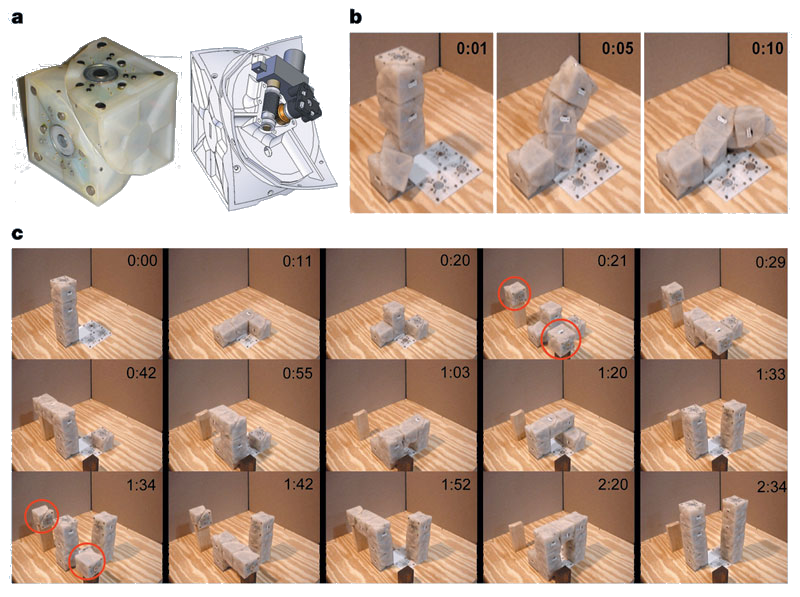
\includegraphics[width=\textwidth]{molecubes}}
	 {\caption{Molecubes (from \cite{zykov_self-reproducing_2005})}
	 \label{fig:mole}}
\end{figure}

The robot consists of modules of 10cm cube, of which the two halves can rotate about the long diagnose(see figure \ref{fig:mole}a). Therefore, each module has one degree of freedom(DOF). The six surfaces of the module are equipped with switchable electromagnet, which can be the state of ``north'', ``south'' and ``off''. Thus, the cubes are able to attract or repel the neighbor cubes. Power and information can also be transmitted to neighbor cubes via adjacent surfaces, that are attached. Multiple modules can be assembled to form a chain-like or other shapes. And, the assembled modules can perform more complicated moves(see figure \ref{fig:mole}b). 

The self-replication process is performed in a highly structured environment with some extent of human assistance. The molecubes are placed on a desk with regular grids. Some of the grids provide the Molecubes with attaching points and 12V power supply. There are also some special grids called ``feeding'' location. At those location, spare modules are replenished. That is the only human intervention during the whole reproduction process.

The replication procedure, namely the sequence of movement, is manually designed. Physical experiments in self-replication of 3-module and 4-module robots were carried out. Figure \ref{fig:mole}c shows the self-replication process of the 4-module robot. The process spans out two and half minutes. At first, the original robot is provided. It moves and places its own module to specific location. Then, it picks up spare module from ``feeding'' locations, which is circled in red in the figure. At the end, the identical replica of the 4-module robot is assembled. Their experiments also show that the replica also seccessfully replicates itself. They also showed their design of replcating seqences for 2n-module ($n > 1$) robots. 

\subsection{Evolved design}
Rather than design the robots shape and replicating sequence manually, Zykov \etal also proposed an evolved design method for 2-D Molecubes in a simulating environment\cite{zykov_evolved_2007}.

The 2-D Molecubes are similar to 3-D Molecubes but the model is 2 dimensional and the modules are of two different types. The two types of the modules are swiveling blocks with permanent magnets and nonswiveling blocks with switchable electromagnet (an ``end-effector''). Like its 3-D version, the swiveling blocks can rotate about it diagnose. An ``end-effector'' are able to take the initiative to attach to another cube.

The evolution algorithm consists of two steps. The first is to evolve the morphology of the machine. As there are millions of combinations and layouts of the modules, the varied morphology of the robot can result in different capability of reaching to surround area. It is neccessary for the robot to reach an area that contains the detacted copy of itself and the ``feeding'' locations.


 

\section{Self-assembly of randomly agitated modules}
\label{sec:random}

\TODO{}

\section{Discussion}
\label{sec:discuss}

\subsection{a}

\TODO{}

%%%%%%%%%%%%%%%%%%%%%%%%%%%%%%%%%%%%%%
% hier werden - zum Ende des Textes - die bibliographischen Referenzen
% eingebunden
%
% Insbesondere stehen die eigentlichen Informationen in der Datei
% ``bib.bib''
%

\bibliography{bib}
\bibliographystyle{plain}
\addcontentsline{toc}{section}{Bibliography}% Add to the TOC

\end{document}
